\chapter{Refactoring}

\section{Code Smells}
\subsection*{Code Comments}
Der erste Code zeigt den Zustand vor dem Refactoring der Klasse 
\textit{LevelGenerator}, mittlerweile \textit{IsaacLevelGenerator}
genannt (Commit 13d1315). Es fallen sofort die ausführlichen Kommentare
auf. Diese stellen einen \textit{Code Smell} dar, weil sie versuchen
eine Erklärung zu liefern für Code, welcher scheinbar selbst nicht
aussagekräftig genug ist.

Dabei war besonders verwirrend, was mit \textit{virtual} gemeint ist.
Folglich wurden die Kommentare, wie im zweiten Snippet zu sehen,
entfernt und die Funktionen entsprechend umbenannt, sodass anhand
der Namen ersichtlich ist, dass es sich hierbei um einen mehrschrittigen
Generierungsprozess handelt, bei dem zunächst Prototypen des Levels
generiert werden (Commit a149b1c). Die Intention ist nun trotz
Kommentare gut verständlich.

\vspace{0.5cm}
\begin{lstlisting}[caption={Code Smell: Code Comments (Vorher)}]
    public static Level generate(Game game, int number) {
        // The generator makes a virtual floor plan based upon an abstract grid.
        // On this grid, small rooms are placed and connected to their direct
        // neighbors.
        VirtualCellFloorPlan cellPlan = LevelGenerator.generateVirtualFloorPlan();
        
        // The small rooms are then aggregated to bigger rooms. However, the spawn
        // and boss room are excluded from that operation. Exits of former small
        // rooms (now sections of bigger rooms) are preserved if they point into
        // another room. Otherwise, they are discarded. The abstraction is still
        // based on the grid.
        VirtualAggregateFloorPlan aggregatePlan = LevelGenerator.aggregate(cellPlan);
        
        // Based on the virtual floor plan actual rooms are generated. They are
        // then connected by the virtual exits that are left. This effectively
        // spans up a graph traversable by the player. Furthermore, each door
        // is detached from a grid position and is placed at real room coordinates.
        MaterializedFloorPlan materializedPlan = LevelGenerator.materialize(aggregatePlan, game.getPlayer());
        
        // Lastly, the materialized rooms are populated by items and enemies.
        // The rarity of former and the strength of latter is determined by the
        // current floor level.
        LevelGenerator.populate(materializedPlan.getRooms());
        return new Level(number, game.getPlayer(), materializedPlan.getSpawnRoom());
    }
\end{lstlisting}

\vspace{0.5cm}
\begin{lstlisting}[caption={Code Smell: Code Comments (Nachher)}]
    public Level next() {
        PrototypicBasicFloorPlan basicFloorPlan = generatePrototypicBasicFloorPlan();
        PrototypicAggregatedFloorPlan aggregatedFloorPlan = aggregate(basicFloorPlan);
        MaterializedFloorPlan materializedFloorPlan = this.materialize(aggregatedFloorPlan);
        
        LevelGenerator.populate(materializedFloorPlan.getRooms());
        Level result = new Level(this.stage, game.getPlayer(), materializedFloorPlan.getSpawnRoom());
        this.stage++;
        return result;
    }
\end{lstlisting}

\subsection*{Large Class}
Der erste Code zeigt den Zustand vor dem Refactoring der Klasse 
\textit{LevelGenerator}, mittlerweile \textit{IsaacLevelGenerator}
genannt (Commit 1519579). Er zeigt ein Beispiel für den Code Smell
\textit{Large Class}. Die Klasse ist viel zu umfangreich, denn ihr
eigentliches Ziel ist es eine Generatorfunktion für Level bereitzustellen.
Tatsächlich macht sie das und enthält noch zusätzlich einige Methoden
zur Befüllung der Level mit Gegnern und Items. Dies ist jedoch ein
Zwischenstand. Zuvor gab es entsprechende Helferfunktionen auch noch
für die Schritte davor.

Daher wurden zusammengehörige Funktionen, welche sich mit der
Population beschäftigen, in eine andere Klasse namens
\textit{PopulatedFloorPlan} umgezogen (Commit 86490a6). Die
Implementation dieser Klasse sei hier erspart.

Die Hauptklasse \textit{LevelGenerator} ist dadurch sehr viel kleiner
geworden, was die Wartbarkeit und Leserlichkeit erhöht. Ihre einzige
Kernkompetenz, das Generieren von Leveln mittels der
\textit{next()}-Funktion bleibt erhalten.

\vspace{0.5cm}
\begin{lstlisting}[caption={Code Smell: Large Class (Vorher)}]
    public Level next() {
        PrototypicBasicFloorPlan basic = PrototypicBasicFloorPlan.make();
        PrototypicAggregatedFloorPlan aggregated = PrototypicAggregatedFloorPlan.from(basic);
        MaterializedFloorPlan materialized = MaterializedFloorPlan.from(aggregated, this.game);
        
        // LevelGenerator.populate(materializedFloorPlan.getRooms());
        Level result = new Level(this.stage, game.getPlayer(), null);
        this.stage++;
        return result;
    }
    
    private static void populate(Set<Room> rooms) {
        final int enemyRoomCount = (int) (rooms.size() * LevelGenerator.ENEMY_POPULATION_RATIO);
        final int itemRoomCount = (int) (rooms.size() * LevelGenerator.ITEM_POPULATION_RATIO);
        CollectionSelector<Room> range = new CollectionSelector<>(new ArrayList<>(rooms));
        List<Room> enemyRooms = range.random(enemyRoomCount).get();
        List<Room> itemRooms = range.random(itemRoomCount).get();
        
        LevelGenerator.populateWithEnemies(enemyRooms);
        LevelGenerator.populateWithItems(itemRooms);
    }
    
    private static void populateWithEnemies(List<Room> enemyRooms) {
        List<LivingEntityType> entityTypes = new ArrayList<>(List.of(LivingEntityType.values()));
        entityTypes.remove(LivingEntityType.PLAYER);
        CollectionSelector entityTypesRange = new CollectionSelector(entityTypes);
        //int maxEnemyCount = Game.getInstance().getStage();
        int maxEnemyCount = 1;
        
        enemyRooms.forEach(room -> {
            int enemyCount = IntRange.from(1, maxEnemyCount).random();
            for (int i = 0; i < enemyCount; i++) {
                LivingEntityType type = (LivingEntityType) entityTypesRange.random(1).get().get(0);
                RoomPosition free = room.getRandomOccupiablePosition();
    
                Enemy enemy = new Enemy(free, type);
                room.addEnemy(enemy);
            }
        });
    }
    
    private static void populateWithItems(List<Room> itemRooms) {
        itemRooms.forEach(room -> {
            RoomPosition free = room.getRandomOccupiablePosition();
            boolean consumable = (IntRange.from(0, 1).random() == 1);
            Item item;
            
            if (consumable) {
                boolean heart = (IntRange.from(0, 1).random() == 1);
                if (heart) {
                    item = new HeartItem(free);
                } else {
                    item = new CoinItem(free);
                }
            } else {
                boolean weapon = (IntRange.from(0, 1).random() == 1);
                if (weapon) {
                    CollectionSelector weaponTypesRange = new CollectionSelector(List.of(WeaponType.values()));
                    WeaponType type = (WeaponType) weaponTypesRange.random(1).get().get(0);
                    item = new WeaponItem(free, type);
                } else {
                    CollectionSelector armorTypeRange = new CollectionSelector(List.of(ArmorType.values()));
                    ArmorType type = (ArmorType) armorTypeRange.random(1).get().get(0);
                    item = new ArmorItem(free, type);
                }
            }
            
            room.addItem(item);
        });
    }
\end{lstlisting}

\vspace{0.5cm}
\begin{lstlisting}[caption={Code Smell: Large Class (Nachher)}]
    public Level next() {
        PrototypicBasicFloorPlan basic = PrototypicBasicFloorPlan.make();
        PrototypicAggregatedFloorPlan aggregated = PrototypicAggregatedFloorPlan.from(basic);
        MaterializedFloorPlan materialized = MaterializedFloorPlan.from(aggregated, this.game);
        PopulatedFloorPlan populated = PopulatedFloorPlan.from(materialized, this.game);
        
        Level result = new Level(this.stage, game.getPlayer(), populated.getSpawnRoom());
        this.stage += 1;
        
        return result;
    }
\end{lstlisting}

\section{Refactorings}
\subsection*{Extract Method}
Der erste Code und das erste UML-Diagramm zeigen den Zustand vor
dem Refactoring der Klasse Buffer (Commit 8ed9fae). Der \textit{Buffer}
besitzt eine Zeichen-Matrix der Maße \texttt{width * height} und
eine Farb-Matrix der gleichen Größe. In \textit{toString()} soll mit
diesen Informationen ein String mit den gleichen Maßen erstellt werden.
Dabei wird jedes Element der Zeichen-Matrix mit der entsprechenden
Farbe konkateniert. Es gibt \texttt{height} Zeilen, welche letztlich
zu einem \textit{block} zusammengesetzt werden. Das Ergebnis ist ein
String, welcher den Inhalt des Buffers darstellen kann.

Wie zu sehen, ist der Code allerdings nicht übersichtlich - durch
kurze Variablenbenennung und Verschachtelungstiefe. Wie im zweiten
Code erkennbar (Commit 2adfff4), ist der Code schon lesbarer geworden.
Die \textit{appendCellToString()}-Funktion extrahiert die Logik
zum Beschreiben des Strings, welche zuvor die Schachtelungstiefe
und Komplexität erhöht hat. In der \textit{toString()}-Funktion
wird nun lediglich die Iteration über die Matrizen vorgenommen,
welche sich allerdings auf zwei Schleifen beschränkt. Zudem sind
im gleichen Zuge kleine Veränderungen an \textit{toString()}
vorgenommen worden.

Insgesamt hat die Extraktion in die \textit{appendCellToString()}-Funktion
die Leserlichkeit und Verständlichkeit der \textit(toString())-Funktion
maßgeblich erhöht.

\vspace{0.5cm}
\begin{lstlisting}[caption={Refactorings: Extract Method (Vorher)}]
    @Override
    public String toString() {
        boolean colored = false;
        StringBuilder block = new StringBuilder();
        StringBuilder line = new StringBuilder();
        
        for (int h = 0; h < this.symbols.length; h++) {
            char[] horizontal = this.symbols[h];
            for (int w = 0; w < horizontal.length; w++) {
                String color = this.colors[h][w];
                if (color != null) {
                    line.append(color);
                    colored = true;
                } else if (colored) {
                    line.append(ANSIColor.RESET);
                    colored = false;
                }
                
                char symbol = horizontal[w];
                line.append(symbol);
            }
            
            block.append(line);
            block.append("\n");
            line.setLength(0);
        }
        
        return block.toString();
    }
\end{lstlisting}

\vspace{0.5cm}
\begin{figure}[H]
    \centering
    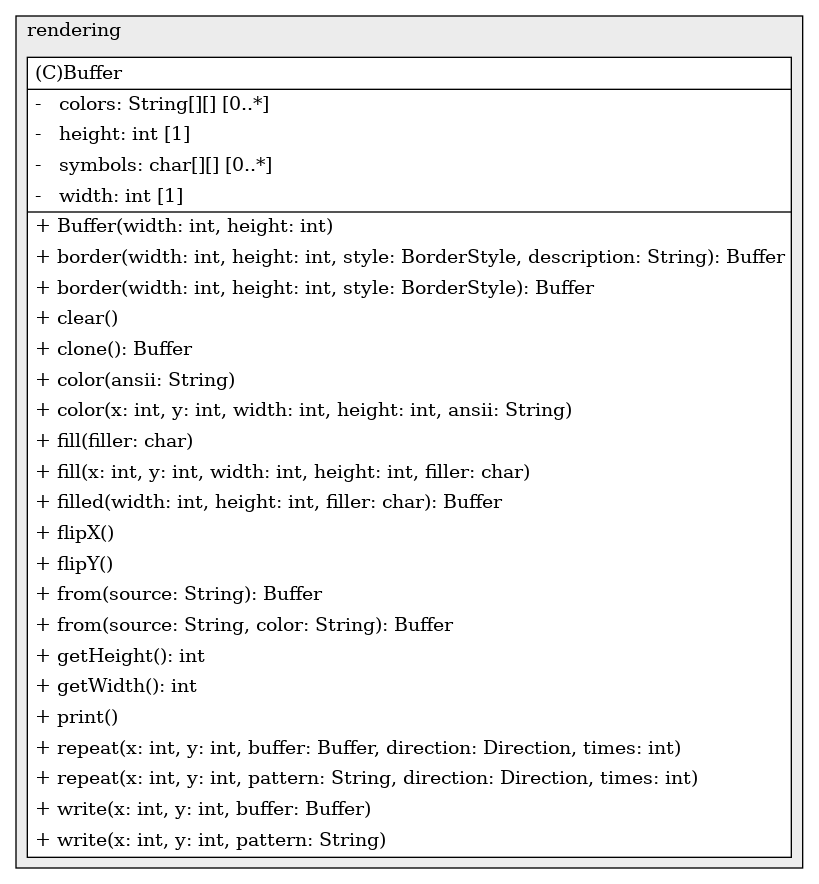
\includegraphics[width=0.6\linewidth]{Bilder/Visualisierung/BufferBeforeRefactor_structure.png}
    \caption{Refactorings: Extract Method (Vorher)}
\end{figure}

\vspace{0.5cm}
\begin{lstlisting}[caption={Refactorings: Extract Method (Nachher)}]
    private void appendCellToString(int x, int y, StringBuilder result) {
        String color = this.colors[y][x];
        if (color != null) {
            result.append(color);
        }
        
        result.append(this.symbols[y][x]);
        
        if (color != null) {
            result.append(ANSIColor.RESET);
        }
    }
    
    @Override
    public String toString() {
        StringBuilder result = new StringBuilder();
        for (int h = 0; h < this.symbols.length; h++) {
            for (int w = 0; w < this.symbols[h].length; w++) {
                this.appendCellToString(w, h, result);
            }
            
            result.append("\n");
        }
        
        return result.toString();
    }
\end{lstlisting}

\vspace{0.5cm}
\begin{figure}[H]
    \centering
    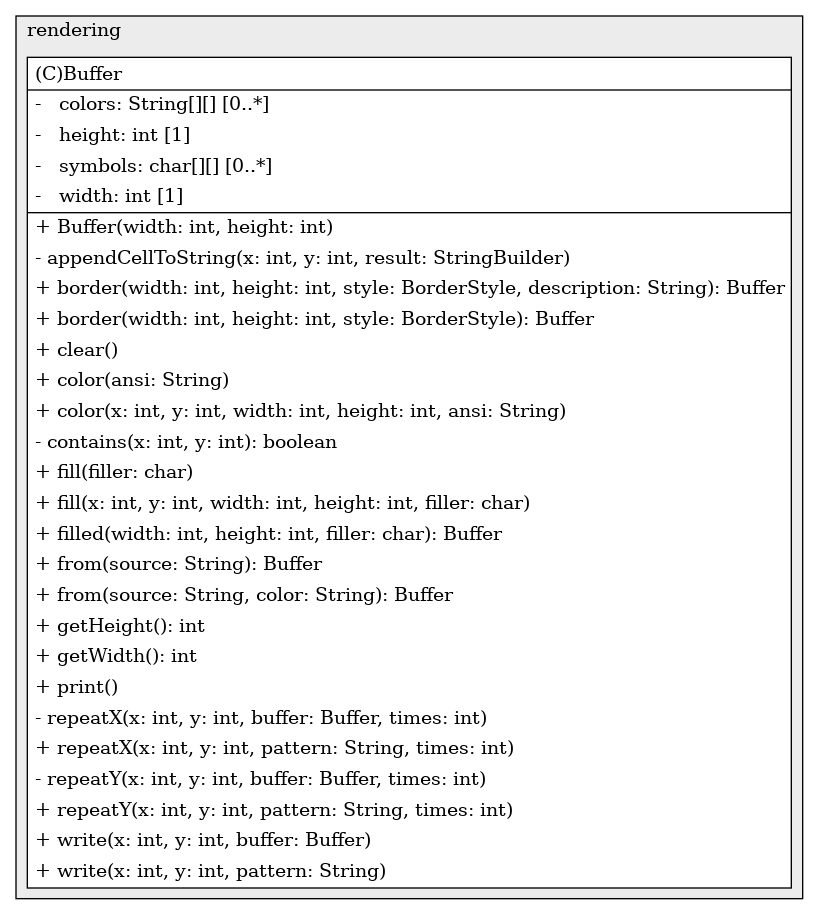
\includegraphics[width=0.6\linewidth]{Bilder/Visualisierung/BufferAfterRestructure_structure.png}
    \caption{Refactorings: Extract Method (Nachher)}
\end{figure}

\subsection*{Rename Method}
Der erste Code und das erste UML-Diagramm zeigen den Zustand vor
dem Refactoring der Klasse \textit{CompositeBuffer} (Commit 3174f95).
Dabei ist zu sehen, dass die \textit{place()}-Funktion
mit einer Liste namens \textit{fixedComponents} interagiert. Hier
scheint es um fixierte \textit{Buffer} zu gehen, was der Funktionsname
aber nicht zum Ausdruck bringt. Dabei ist \textit{place()} ein
Platzhaltername gewesen. Der Name ist nicht sonderlich aussagekräftig.
Es wird keine Aussage darüber getroffen, \textbf{wie} oder \textbf{unter
welchen Annahmen} ein \textit{Buffer} platziert wird.

Es ist für den zusammengesetzten Buffer (\textit{CompositeBuffer})
angedacht, sowohl fixierte als auch dynamische Elemente zu beherbergen.
Für beide Typen soll es getrennte Funktionen geben, welche namentlich
aussagen sollen, um welchen Platzierungstypen es sich handelt.

Der zweite Code und das zweite UML-Diagramm zeigen den Zustand nach
der Umbenennung (Commit d3307da). Zu sehen ist, dass \textit{place()}
umbenannt wurde in \textit{fixed()}. Dies lässt auch direkt eine
entsprechende \textit{dynamic()}-Funktion zu, welche hier aber noch
nicht implementiert ist. Im Übrigen ist im Bezug auf \textit{fixed()}
noch eine kleine Vereinfachung vorgenommen worden.

Nun ist ersichtlicher, dass es hierbei um die Platzierung fixierter
Elemente geht. Der Funktionsname ist bewusst kurz gewählt, weil
die Parameter zur Konfiguration der Elemente dienen. Diese können
schnell ausarten. Um mehr Übersichtlichkeit zu schaffen, wurde eine
kurze und prägnante Benennung gewählt, ähnlich dem Benennungstil,
welchen man aus der \textit{Java Stream API} oder von \textit{Buildern}
kennt. Ansonsten bietet \textit{CompositeBuffer} keine weiteren
Funktionen an, was die kurze Benennung ermöglicht, ohne dass
Bedeutungskonflikte auftreten.

\vspace{0.5cm}
\begin{lstlisting}[caption={Refactorings: Rename Method (Vorher)}]
public class CompositeBuffer extends Buffer {
    
    private final List<Buffer> fixedComponents;
    private final Map<Buffer, Position> positions;
    private final char background;
    
    public CompositeBuffer(int width, int height, char background) {
        super(width, height);
        this.fixedComponents = new ArrayList<>();
        this.positions = new HashMap<>();
        this.background = background;
    }
    
    public CompositeBuffer(int width, int height) {
        this(width, height, ' ');
    }
    
    public void place(Buffer buffer, int x, int y) {
        this.fixedComponents.add(buffer);
        this.positions.put(buffer, new Position(x, y));
    }
    
    public void render() {
        this.fill(this.background);
        this.color(ANSIColor.RESET);
        
        for (Buffer component : this.fixedComponents) {
            component.render();
            this.write(this.positions.get(component), component);
        }
    }
    
}
\end{lstlisting}

\vspace{0.5cm}
\begin{figure}[H]
    \centering
    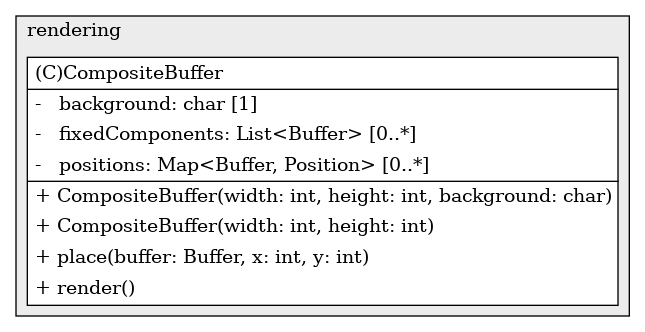
\includegraphics[width=0.6\linewidth]{Bilder/Visualisierung/CompositeBufferPlaceFunction_structure.png}
    \caption{Refactorings: Rename Method (Vorher)}
\end{figure}

\vspace{0.5cm}
\begin{lstlisting}[caption={Refactorings: Rename Method (Nachher)}]
public class CompositeBuffer extends Buffer {
    
    private final Map<Buffer, Position> fixed;
    private final char background;
    
    public CompositeBuffer(int width, int height, char background) {
        super(width, height);
        this.fixed = new LinkedHashMap<>();
        this.background = background;
    }
    
    public CompositeBuffer(int width, int height) {
        this(width, height, ' ');
    }
    
    public void fixed(Buffer buffer, int x, int y) {
        this.fixed.put(buffer, new Position(x, y));
    }
    
    public void render() {
        this.fill(this.background);
        this.color(ANSIColor.RESET);
        
        this.fixed.forEach((component, position) -> {
            component.render();
            this.write(position, component);
        });
    }
    
}
\end{lstlisting}

\vspace{0.5cm}
\begin{figure}[H]
    \centering
    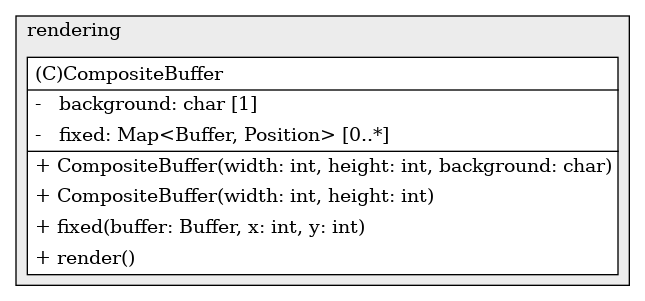
\includegraphics[width=0.6\linewidth]{Bilder/Visualisierung/CompositeBufferFixedFunction_structure.png}
    \caption{Refactorings: Rename Method (Nachher)}
\end{figure}
